\chapter{Preprocesado de datos}


Una vez examinados todos los conjuntos mencionados anteriormente, podemos llevar a cabo la unión de todos los datos en un único subconjunto. Esto nos permitirá conseguir un dataset completo y variado con diferentes tipos de piel y diferentes lesiones que nos permitirán identificar multitud de tipos de patologías, siendo posible ajustar el grado de granularidad en función de la agrupación o no de posibles subclases.

Inicialmente, el conjunto de datos construido contendrá todos los subtipos de lesiones cutáneas vistos, pero dispondrán de una segunda etiqueta que indicará si se trata de un caso canceroso o no, atendiendo a su subclase que lo etiqueta. Si agrupamos por lesiones benignas, cancerosas, y potencialmente cancerosas, podemos obtener el siguiente diagrama de sectores de la figura \ref{tartabinaria}, donde se puede observar cómo la mayoría de imágenes disponibles engloban problemas de piel no cancerosos, mientras que el segundo tipo más común de lesión si es la cancerosa. Si atendemos a clasificar las subclases de cada tipo de patología, encontramos 52 posibles etiquetas, las cuales iremos examinando a medida que se preprocese cada uno de los subconjuntos.


\begin{figure}[H]
	\centering
	\label {tartabinaria}
	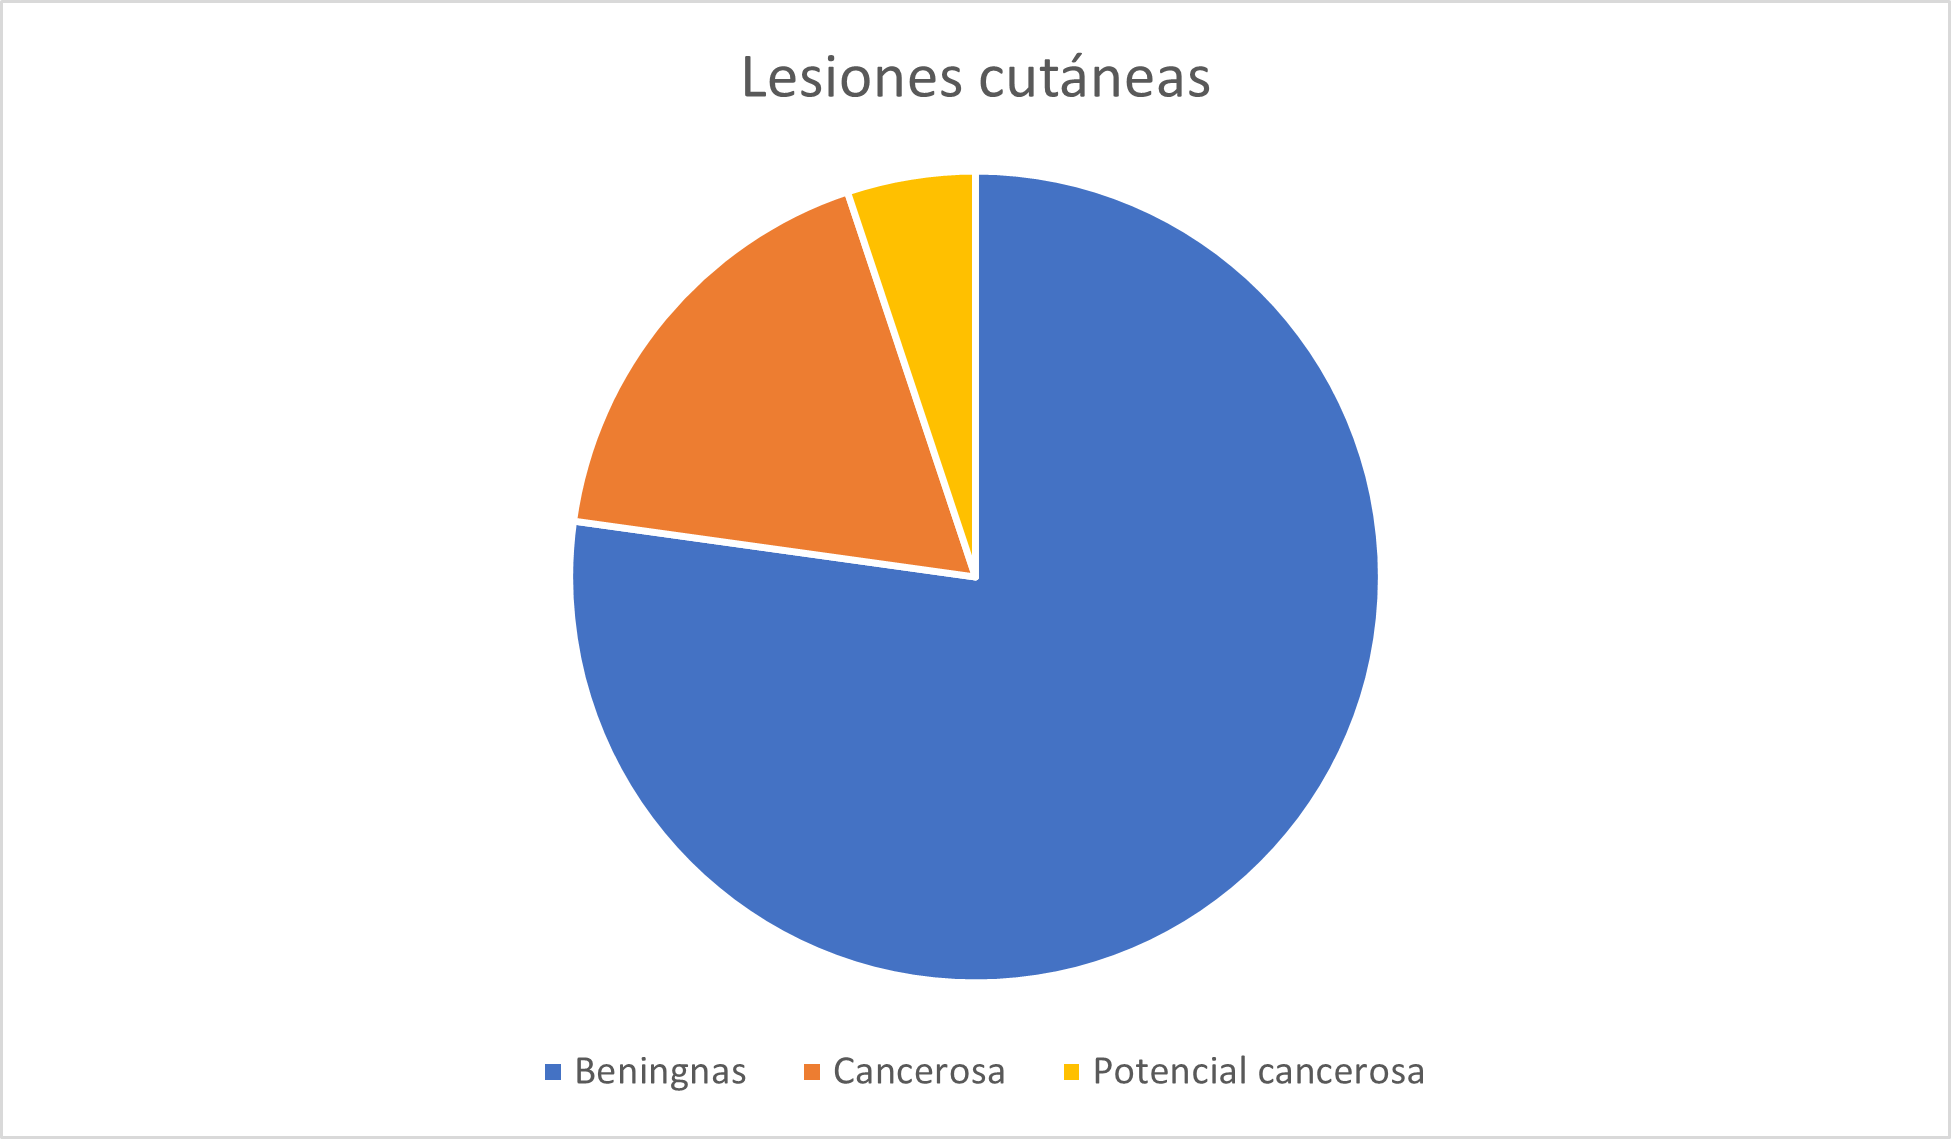
\includegraphics[scale = 0.7]{imagenes/datasetfinal.png}
	\caption{Distribución de clases}
\end{figure}

En el caso de las lesiones potencialmente cancerosas, como se trata de condiciones de la piel no cancerosas con posible evolución a cancerosas, se tendrán en cuenta como imágenes benignas, ya que la condición de malignidad sólo podría aparecer en el futuro, el cual sigue siendo desconocido.


%\section{Procesado de imágenes cutáneas}
 


